In this chapter, we will look at a numerical computing problem that is well
suited to being parallelised, namely to calculate an approximation of a definite
integral:
\[
\int_a^b f(x) \, dx .
\]

%%%%%

\section{The Trapezium Rule}

The trapezium rule is a standard numerical technique to approximate the value
of an integral.  It splits the integral's range $[a,b]$ into $n \ge 1$
intervals:
\[\mstyle
\begin{align}
[{a+i\delta}, a+(i+1)\delta], 
  \quad\mbox{for $i = 0, \ldots, n-1$,} \\
\mbox{where $\delta = (b-a)/n$.}
\end{align}
\]
This is illustrated in Figure~\ref{fig:trapezium} with $n = 4$
(although in practice we would use a much larger value of~$n$).

%%%%%%%%%%%%%%%%

\begin{figure}
\begin{center}
\def\labY{-0.16}
\def\fn{\x^3/240 + \x^2/10 - 0.5*\x + 1.5}   %2.5*\x^2-2*\x+15}
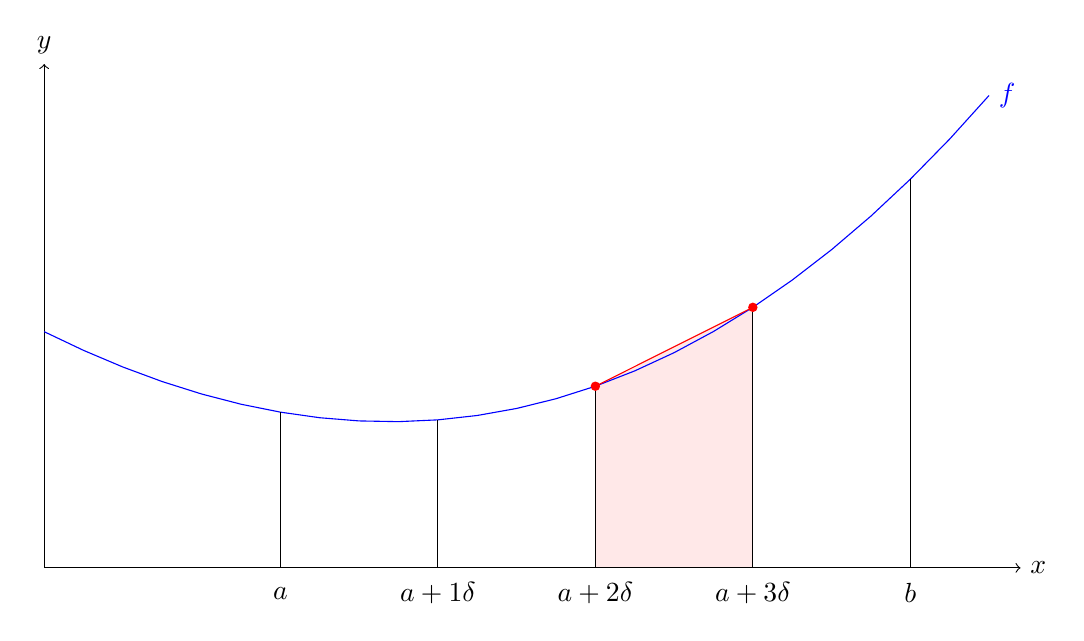
\begin{tikzpicture}[domain=0:6, scale = 2]
% Coordinates of selected points
\foreach \x in {3.5}  \draw (\x,\fn) coordinate (c1); %  node (c1) {};
\foreach \x in {4.5}  \draw (\x,\fn) coordinate (c2) {};
% Fill trapezium
\fill[red!9] (c1) -- (c2) -- (4.5,0) -- (3.5,0) -- (c1);
% Axes
\draw[->] (0,0) -- (6.2,0) node[right] {$x$};
\draw[->] (0,0) -- (0,3.2) node[above] {$y$};
% Plot
\draw[color=blue] plot (\x,\fn) node[right] {$f$}; 
% x labels
\draw(1.5,\labY) node{$a$};
\foreach \x in {1,2,3} \draw (\x+1.5,\labY) node{$a+\x \delta$};
\draw (5.5,\labY) node{$b$};
% Verticals
%\foreach \i in {0,1,2,3,4} \foreach \x in {\i+1.5} 
\foreach \x in {1.5,2.5,3.5,4.5,5.5} 
  \draw (\x,0) -- (\x,\fn);
% Blobs at selected points, and line between them
\draw[red] (c1) -- (c2);
\fill[red] (c1) circle[radius = 0.3mm];
\fill[red] (c2) circle[radius = 0.3mm];
\end{tikzpicture}
\end{center}
\caption{Illustration of the trapezium rule}
\label{fig:trapezium}
\end{figure}

%%%%%

The integral over the interval $[a+i\delta, a+(i+1)\delta]$ can then be
approximated by 
\[\mstyle
\frac{f(a+i\delta)+f(a+(i+1)\delta)}{2} \times \delta.
\]
In other words, we approximate the graph of the function over this interval by
a straight line between the endpoints.  This is illustrated in
Figure~\ref{fig:trapezium} for the interval $[a+2\delta, a+3\delta]$.  The red
blobs give the values of the function at the endpoints; the function is
approximated by the red line; and so the integral is approximated by the area
of the pink region.  For this interval, the approach gives a slight
overapproximation. 

Summing over all intervals then gives us the following approximation:
\begin{eqnarray*}
\int_a^b f(x) \, dx  & = & 
  \sum_{i = 0}^{n-1} \int_{a+i\delta}^{a+(i+1)\delta} f(x)\, dx \\
& \approx & 
  \sum_{i=0}^{n-1} \frac{f(a+i\delta) + f(a+(i+1)\delta)}{2} \times \delta \\
& = &
  \left( \frac{f(a)+f(b)}{2} + \sum_{i=1}^{n-1} f(a+i\delta) \right) \times \delta.
\end{eqnarray*}

Figure~\ref{fig:trapezium-sequential} gives straightforward sequential code to
implement the trapezium rule\footnote{The type {\scalashape Double
    \protect\SCALA{=>} Double} represents functions from {\scalashape Double}
  to {\scalashape Double}.}.  (We will see several implementations of the
trapezium rule, so we factor out some common code into an abstract class
|TrapeziumT|.)

%%%%%

\begin{figure}
\begin{scala}
/** Abstract class representing the problem of approximating the integral of £f£
  * from £a£ to £b£. */
abstract class TrapeziumT(f: Double => Double, a: Double, b: Double){
  /** Calculate the integral. */
  def apply(): Double

  /** Use trapezium rule to approximate the integral of £f£ from £left£ to £right£, 
    * using £n£ intervals of size £delta£. 
    * Precondition: £n*delta = right-left£ (modulo rounding errors). */
  protected 
  def integral(left: Double, right: Double, n: Int, delta: Double): Double = {
    require(n > 0 && Math.abs(n*delta-(right-left)) < 0.000000001) 
    var sum: Double=(f(right)+f(left))/2.0
    for(i <- 1 until n) sum += f(left+i*delta)
    sum*delta
  }
}

/** Approximation of the integral of £f£ from £a£ to £b£, using a sequential 
  * implementation of the trapezium rule. */
class SeqTrapezium(f: Double => Double, a: Double, b: Double, n: Int)
    extends TrapeziumT(f, a, b){
  require(n > 0)

  def apply() = integral(a, b, n, (b-a)/n)
}
\end{scala}
\caption{Sequential code to apply the trapezium rule.}
\label{fig:trapezium-sequential}
\end{figure}

%%%%%%%%%%%%%%%%%%%%%%%%%%%%%%%%%%%%%%%%%%%%%%%%%%%%%%%%%%%%

\section{A parallel implementation}

Here is the idea of a parallel implementation.  We use some number |nWorkers|
of \emph{worker threads}.  We then split the interval $[a,b]$ into the same
number of equal-size subranges, so each worker works on one subrange.  A
\emph{controller} thread tells each worker which subrange to work on.  Each
worker sends its subresult back to the controller, which adds them up to give
the overall result.

This is a form of \emph{data parallelism}.  We split the data (the value
of~$f$ over the relevant range) between the workers.  Each worker calculates a
subresult on its part of the data, and then we combine the subresults. 

%%%%%

We will use a channel \SCALA{toWorkers} to communicate from the
controller to the workers, and a channel \SCALA{toController}
to communicate from the workers to the controller.  This is illustrated below.
%
\begin{center}
%\tikzstyle{every node}=[minimum width=5mm,minimum height = 15mm]
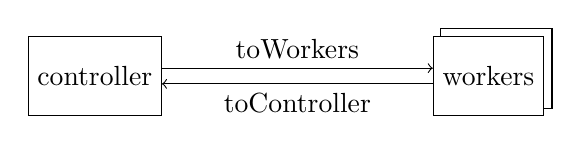
\begin{tikzpicture}
\draw (0,0) node[draw, minimum height = 10mm](c){\scalashape controller};
\draw (5,0) node[draw, minimum height = 10mm] (w){\scalashape workers};
\draw ([xshift = 1mm] w.north west) -- ++ (0,1mm) -- 
  ([xshift = 1mm, yshift = 1mm] w.north east) -- 
  ([xshift = 1mm, yshift = 1mm] w.south east) -- 
  ([yshift = 1mm] w.south east) ;
\draw[->] ([yshift = 1mm] c.east) -- node[above]{\scalashape toWorkers} 
  ([yshift = 1mm] w.west);
\draw[<-] ([yshift = -1mm] c.east) -- node[below]{\scalashape toController} 
  ([yshift = -1mm] w.west);
\end{tikzpicture}
\end{center}

In examples so far, each channel has had one sender and one receiver.
However, an in-port or out-port may be shared between any number of receivers
or senders.  Here, it is useful for the controller to use a single channel to
send to all the workers, and likewise to use a single channel to receive
subresults from all the workers.

Figure~\ref{fig:trapezium-1} gives some of the code.  The companion object
|Trapezium| factors out some definitions that we will reuse in a later
implementation.  (We take the parameter |n| of |Trapezium|---the number of
intervals---to be a |Long|, because we want to experiment with large
arguments; in practice, an |Int| would be large enough.)

%%%%%

\begin{figure}
\begin{scala}
/** Companion object, collecting some code that is common across 
  * implementations. */
object Trapezium{
  /** Type of tasks to send to client.  The Task £(left, right, taskSize, delta)£
    * represents the task of calculating the integral from £left£ to £right£,
    * using £taskSize£ intervals of size £delta£. */
  type Task = (Double, Double, Int, Double)

  /** Make a channel, based on the value of `buffering`. */
  def mkChan[A: scala.reflect.ClassTag](buffering: Int): Chan[A] = 
    if(buffering == 0) new SyncChan[A] 
    else if(buffering == 1) new OnePlaceBuffChan[A]
    else if(buffering > 1) new BuffChan[A](buffering) 
    else new UnboundedBuffChan[A]
}

/** Parallel implementation of the trapezium rule. */
class Trapezium(
  f: Double => Double, a: Double, b: Double, 
  n: Long, nWorkers: Int, buffering: Int = 0)
    extends TrapeziumT(f, a, b){
  require(n >= nWorkers)

  import Trapezium.{Task, mkChan}

  /** Channel from the controller to the workers, to distribute tasks. */
  private val toWorkers: Chan[Task] = mkChan[Task](buffering)

  /** Channel from the workers to the controller, to return subresults. */
  private val toController: Chan[Double] = mkChan[Double](buffering)

  /** A worker, which receives arguments from the controller, estimates the
    * integral, and returns the results. */
  private def worker = thread("worker"){
    val (left, right, taskSize, delta) = toWorkers?()
    val result = integral(left, right, taskSize, delta)
    toController!result
  }
  ...
}
\end{scala}
\caption{Parallel implementation of the trapezium rule (part 1).}
\label{fig:trapezium-1}
\end{figure}

%%%%%

We want to experiment to see whether using buffered channels is advantageous.
We use the function~|mkChan| to make a channel passing data of type~|A|, where
the parameter |buffering| indicates the amount of buffering, with |0|
indicating a synchronous channel, and a negative value indicating an unbounded
buffered channel.

The controller needs to tell each worker the range \SCALA{[l,r]} to work on,
the number \SCALA{taskSize} of intervals in its range, and the size
\SCALA{delta} of each interval (so $\sm{taskSize} \times \sm{delta} \approx
\sm{r} - \sm{l}$).  We can pass this information as a 4-tuple \SCALA{(l, r,
  taskSize, delta)}.  We define a type |Task| to represent such 4-tuples, and
create a channel |toWorkers| to pass |Task|s.  

Each worker returns a \SCALA{Double} to the controller, so we create a channel
|toController| to pass such values.

The definition of a worker is then straightforward: it receives a task on the
|toWorkers| channel, calculates the approximation to the integral, and sends
the result back on the |toController| channel.

In earlier chapters, we used channels to pass only simple values, such as
|Int|s.  However, |Task|s (like all tuples) are reference objects.  When a
reference object is sent on a channel, the value that is actually passed is a
reference to the object (i.e.~its address in memory): the object itself is not
copied.  This means that even if an object encapsulates a lot of data, it is
not expensive to send on a channel.

%%%%%

\begin{figure}
\begin{scala}
  /** This variable ends up holding the result. */
  private var result = 0.0

  /** A controller, who distributes tasks to the clients, and accumulates the
    * subresults into £result£. */
  private def controller = thread("controller"){
    val delta = (b-a)/n    // Size of each interval.
    var remainingIntervals = n    // Number of intervals not yet allocated.
    var left = a // Left-hand boundary of the next task.
    for(i <- 0 until nWorkers){
      // Number of intervals in the next task; £$\lceil \sm{remainingIntervals/(nWorkers-i)} \rceil$£.
      val taskSize = ((remainingIntervals-1) / (nWorkers-i) + 1).toInt
      remainingIntervals -= taskSize; val right = left+taskSize*delta
      toWorkers!(left, right, taskSize, delta); left = right
    }

    // Receive results, and add them up.
    result = 0.0
    for(i <- 0 until nWorkers) result += toController?()
  }    
    
  /** The main system. */
  private def system = {
    val workers = || (for (i <- 0 until nWorkers) yield worker)
    workers || controller
  }

  /** Calculate the integral, and return the result. */
  def apply(): Double = { run(system); result } 
\end{scala}
\caption{Parallel implementation of the trapezium rule (part 2).}
\label{fig:trapezium-2}
\end{figure}

%%%%% Controller

We now consider the controller (given in Figure~\ref{fig:trapezium-2}).  We do
not assume that |n| (the number of intervals) is divisible by |nWorkers| (the
number of workers); instead, workers might receive slightly different size
tasks (but differing by at most one interval).  More precisely, the code
maintains a variable |remainingIntervals| that represents the number of
intervals still to allocate.  In the first loop, |nWorkers-i| represents the
number of tasks to send.  Then the next task contains $\lceil
\sm{remainingIntervals/(nWorkers-i)} \rceil$ intervals, i.e.~rounding up the
average; the expression defining |taskSize| calculates this using integer
arithmetic: the ``|/|'' is integer division.  (The final ``|toInt|'' is
necessary only because we took |n| to be a |Long|, and so the result of the
division is also a |Long|.)

The second loop in the controller receives subresults from the workers, 
and accumulates them into the object variable |result|.

The function |system| constructs the system.  The definition of |workers|
builds a sequence of workers using a |for| expression (see Scala
box~\ref{sb:for-expression}).  It then combines them together in parallel
using an indexed form of parallel composition: if |ts| is a sequence of
|ThreadGroup|s, then \SCALA{\|\| ts} represents their parallel composition,
and is itself a |ThreadGroup|.

\framebox{for expressions}

Finally, the |apply| function runs the system and returns the final result
from the |result| variable. 

%%%%%%%%%%

\section{Testing}

We now consider how to test the concurrent implementation.  The obvious
approach is to run both the sequential and concurrent implementations on the
same integral, and test whether they give the same result.  In particular, my
approach was to generate random polynomials for the function~|f| to integrate,
and random values for |a|, |b|, |n| and |numWorkers| (within sensible ranges).
We can then run many such tests.

However, it turns out that this approach doesn't quite work.  If we use both
implementations to approximate $\int_0^3 x^2 \mbox{d}x$ using $100$ intervals,
the sequential algorithm always gives
\[\mstyle
  9.000449999999995.
\]
However,  the concurrent implementation with 10 workers normally gives
\[\mstyle
  9.000449999999999,
\]
but sometimes gives
\[\mstyle
  9.000449999999997.
\]

%%%%%

The difference in results can be explained by rounding errors, and in
particular that machine addition is not associative (you can verify this by
getting Scala to evaluate the expressions |(1E10 + (-1E10)) + 1E-10| and
\SCALA{1E10 + (-1E10 + 1E-10)}: the former gives the expected result, but the
latter evaluates to |0.0|, because rounding errors in the right-hand addition
cause the final term to be lost).
%
In the sequential algorithm, the values for the intervals are added up from
left to right.  But in the concurrent algorithm, they are added up in a
different order, giving a different result.  Further, in different runs of the
concurrent algorithm, the subresults are returned to the controller in
different orders, and so added up in different orders, giving different
results.

%%%%%

Instead, we can compare whether sequential result |seqResult| and the
concurrent result |concResult| are approximately equal using a test such as
\begin{scala}
  assert(
    seqResult != 0.0 && Math.abs((seqResult-concResult)/seqResult) < 1E-7 ||
      Math.abs(seqResult-concResult) < 1E-10, ...)
\end{scala}
%
The second clause tests whether the relative error is less than one part
in~$10^7$; the first clause guards against division by~$0$; the third clause
is necessary to cover the case where both the sequential and concurrent
results are small, the relative error isn't quite small enough to satisfy the
second clause, but the absolute error is very small.  (I originally omitted
the third clause, but one test produced a false error.)  If this test passes,
we can be pretty confident that any difference between |seqResult| and
|concResult| is caused only by rounding errors.

Incidentally, when I first ran these tests, they threw up other false errors,
because I hadn't thought carefully enough about preconditions of different
parts of the code.  For example, I hadn't realised that the |integral|
function (Figure~\ref{fig:trapezium-sequential}) requires a precondition
\SCALA{n > 0} (or else it gives an incorrect result); and hence the |Trapezium|
class (Figure~\ref{fig:trapezium-1}) requires a precondition |n >= nWorkers|
(or else a worker will receive an empty task).  
